
\chapter{基于多帧散斑照明的散射介质3D目标成像}

在前面章节中,我们对基于OME卷积成像模型进行了介绍,通过数值仿真和实验验证的方式,对散斑自相关的基本成像原理进行研究,研究了不同相位恢复算法的特点实现透过散射介质彩色成像和基于散斑的之间相的关性提出新型的非入侵透过散射介质成像方法。在第\ref{chap:5}章节中,我们所提出的方法能够有效的恢复超出光学记忆的目标,实现了对于扩展目标的非入侵成像。然后,如何有效的实现透过散射介质3D成像仍具有挑战性,以上的方法都具有各自的局限性,无法有效地解决透过散射介质的3D成像。

\begin{figure}[htp]
	\centering
	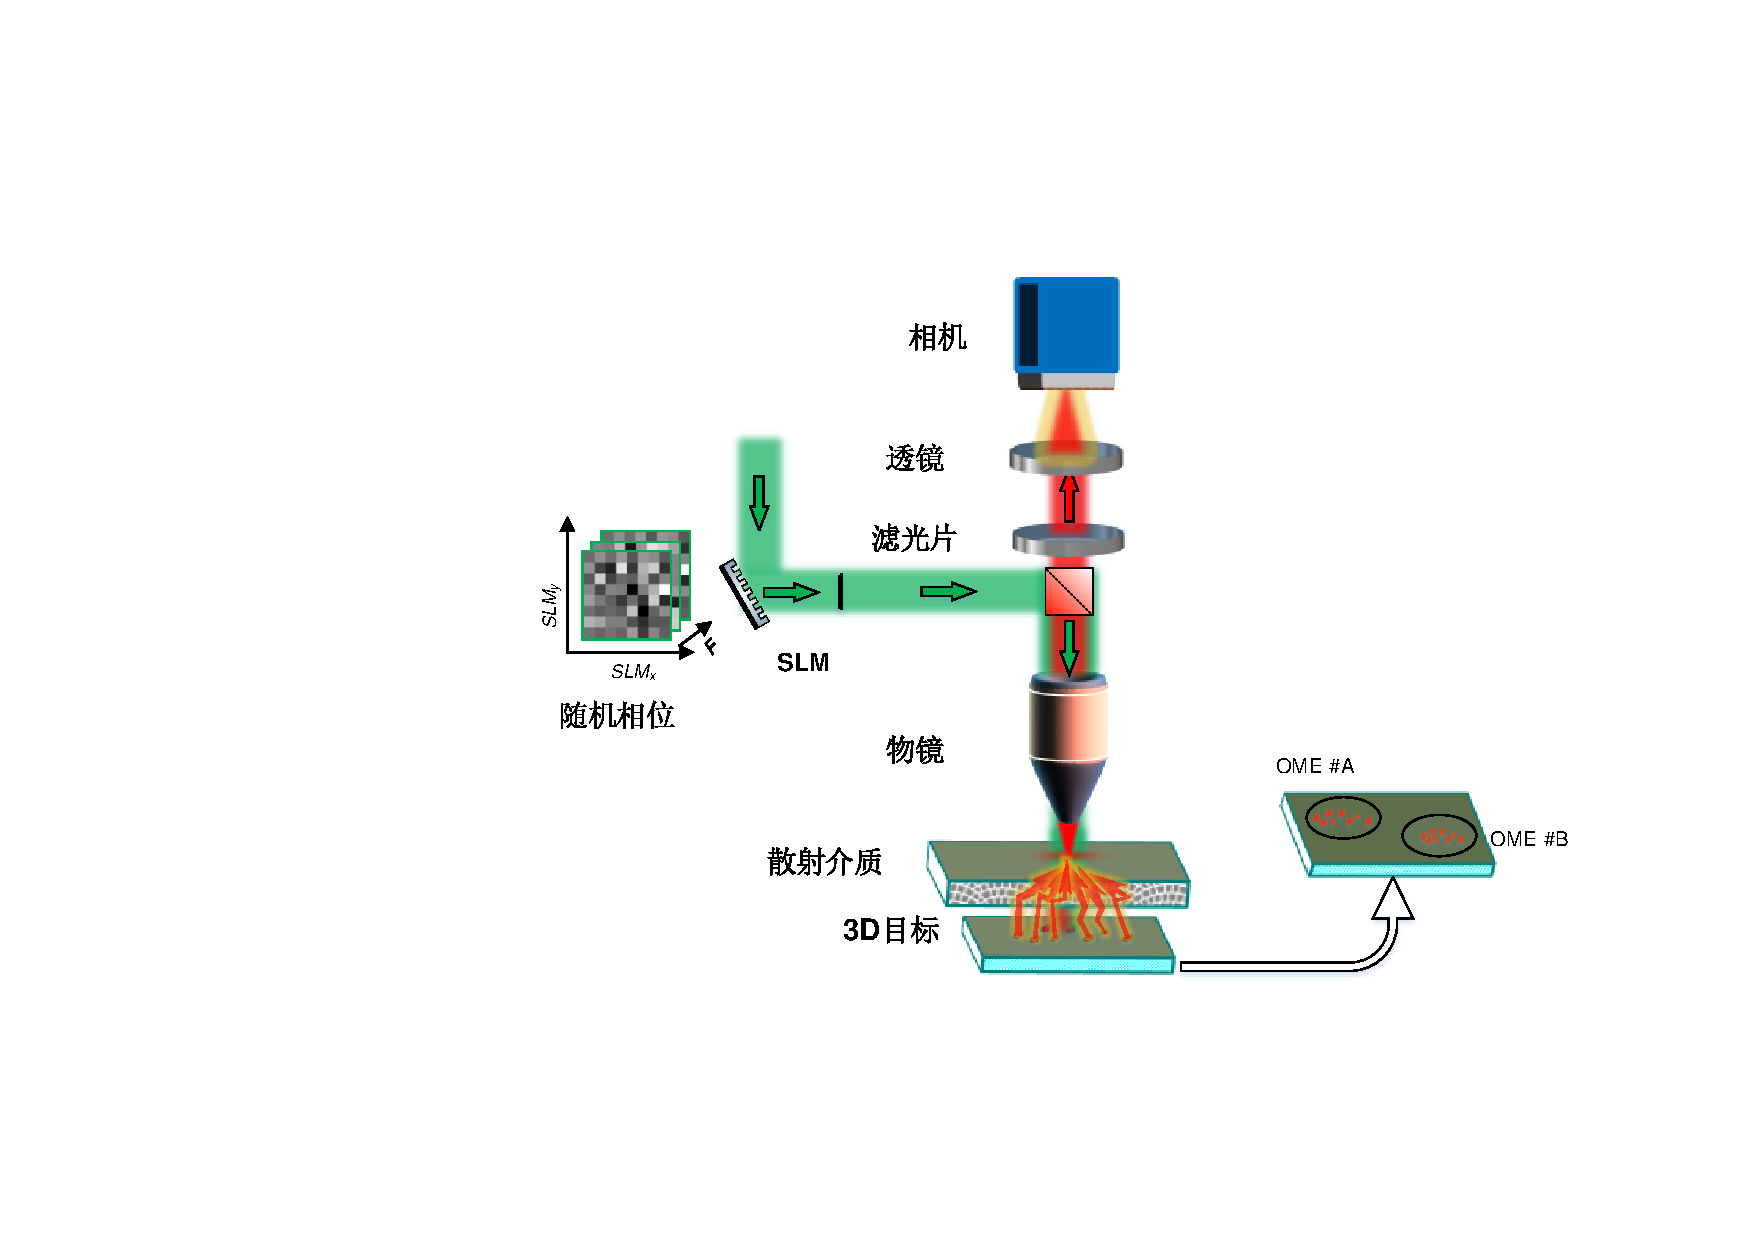
\includegraphics[scale=0.75]{C6.fig1}
	\caption{多帧散斑照明的散射3D目标成像示意图}
	\label{fig:6.1}
\end{figure}

针对透过散射介质进行3D目标成像问题已经进行多年,目前已有的方法可以大致分为以下三个方面:第一,利用散射介质的空间去相关特性,对系统的PSF进行预标定,实现不同景深或者不同视场的图像拼接;第二,利用参考目标或者放置点源目标的方式,然后从复杂信号中提取目标信息并进行图像重建;第三,测量光学传输矩阵,获得更大范围光场的控制,进而实现大视场扫描成像。利用散射介质的先验信息、放置参考目标的方式或者测量光学传输矩阵方法,虽然在一定程度上实现了透过散射介质的大视场或者3D目标成像,但是难以在非入侵的条件下进行实施。与第\ref{chap:5}章节中所展示的结果不同,本章我们重点研究当空间存在多个目标,不同的目标位于不同OME范围,如何进行有效地进行图像重建。受到第\ref{chap:5}章节方法的启发,我们可以通过随机照明的方式,获得系统中不同点光源的散斑指纹,但是当有效的获取散斑指纹后该如何进行重建将在接下来部分进行讨论。同时受到机器学习、图像分类和模式识别相关工作的启发,我们提出了一种非入侵透过散射介质3D目标成像方法,利用随机照明的方式获得散斑图案进行去混叠获得散斑指纹,对散斑指纹进行分类,并最终实现了透过散射介质的3D成像。我们的方法特点在于:(\romannum{1})只需散斑照明;(\romannum{2})无需相位恢复;(\romannum{3})与散斑自相关成像方法相比,能够更好的重建图像,具有较高的图像分辨率。

由于目前针对于散射成像的研究方向更倾向于与生物成像像交叉的方法,同时荧光成像方式在生物成像方面有着更多的应用,因此本章所描述的成像方法及成像构架均以荧光目标成像为章节主线。然后,我们所提出的方法同样能够扩展至拉曼和多光子成像等领域。

\section{基于多帧散斑照明的散射介质3D目标成像基本原理}

\subsection{3D目标成像模型}

成像系统如图\ref{fig:6.1}所示,当激光通过SLM时,入射激光被添加了随机相位实现调制,进而利用随机散斑照明目标后,目标产生自身的激发光,激发光传播并通过散射介质,产生散斑最终被相机所接收,此时相机所获得的散斑为不同散斑指纹的非相干总和。此外,光学记忆效应范围内的独立点光源将在相机上产生相关但平移的散斑指纹 \cite{Freund1988},而光学记忆效应范围外的点光源将产生完全不相关的散斑指纹。对于给定的散斑照明,捕获的图像 $I_{\textsl{fluo}}$ 可以表示为具有不同权重的散斑指纹的线性叠加。因此,相机图像$I_{\textsl{fluo}}$由下式给出:

\begin{equation}
\begin{aligned}
I_{fluo}(r,t) = \sum^{P}_{k=1} w_{k}(r) h_{k}(t),
\label{eq:6.1}
\end{aligned}
\end{equation}
其中,$I_{fluo}(r,t)$为对应于第$t$次照明时相机所接收到低对比度散斑,$r$为空间坐标,$w_{k}(r)$为第$k$个独立点光源所对应的散斑指纹,$h_{k}(t)$为第$t$次照明时第$k$个独立点光源所接收到的激光光的强度,$P$为系统中独立点光源的数量。

在此成像模型下,假设不同OME范围的PSF已知,图像可以通过简单的去卷积过程进行重建。但是在实际生物成像应用中,获取系散射介质的PSF往往难度较大或者难以实现。受到第\ref{chap:5}章节方法的启发,我们对获得的散斑图像序列利用NMF算法进行去混叠,进而获得不同点光源的散斑指纹。然后,在获得散斑指纹后,如何进行图像重建将是本章的重点。由于去混叠部分与第\ref{chap:5}章节所展示的部分完全相同,所以在此处不进行重复描述。

在此,假设我们的系统中存在目标A和目标B,它们分别位于不同的OEM范围。因此,公式(\ref{eq:6.1})可以写为:
\begin{equation}
\begin{aligned}
I_{fluo}(r,t) = \sum^{P}_{k=1} w_{k}^{A}(r) h_{k}^{A}(t)+\sum^{P}_{k=1} w_{k}^{B}(r) h_{k}^{B}(t),
\label{eq:6.2}
\end{aligned}
\end{equation}
其中,$h_{k}^{A}(t)$和$h_{k}^{B}(t)$分别代表来自目标A和目标B的散斑指纹。假设可以将公式(\ref{eq:6.1})表示为公式(\ref{eq:6.2})的形式,目标A和B分别可以利用第\ref{chap:5}章节所呈现的方法进行重建。

当进行去混叠步骤后,$h_{k}^{A}(t)$和$h_{k}^{B}(t)$被获取,探索不同指纹之间的相关性,将有助于图像重建。受到OME启发,光学记忆效应范围内的独立点光源的散斑指纹之间相关但是之间具有平移\cite{Freund1988},而光学记忆效应范围外的点光源散斑指纹完全不相关。在空间域的位移,在傅里叶域来看的的话,空间的平移对应于频域的斜坡相位,即:
\begin{equation}
\begin{aligned}
\mathcal{F}(h_i^{A}(t)) = \mathcal{F}(h_j^{A}(t))*\mbox{exp}[i\phi_{ramp}]
\label{eq:6.3}
\end{aligned}
\end{equation} 对公式(\ref{eq:6.3})两边同时求绝对值(同傅里叶振幅),即:
\begin{equation}
\begin{aligned}
\mbox{abs} \{ \mathcal{F}(h_i^{A}(t)) \} = \mbox{abs} \{  \mathcal{F}(h_j^{A}(t))*\mbox{exp}[i\phi_{ramp}] \}
\label{eq:6.4}
\end{aligned}
\end{equation}其中,$\mbox{abs}$表示求绝对值运算。

从公式(\ref{eq:6.4})可知,位于同一OME范围内的点光源所对应的散斑指纹的傅里叶变换后,它们的傅里叶振幅接近相等,相关仿真结果如图\ref{fig:6.2}所示。图\ref{fig:6.2}中,(a)和(b)为位于同一OME范围内,不同点光源的散斑指纹;(c)和(d)分别为散斑(a)和(b)的傅里叶变换后的振幅显示;(e)为(c)和(d)图中心切线的强度曲线;(f)和(g)为位于同一OME范围内,不同点光源的散斑指纹;(h)和(i)分别为散斑(f)和(g)的傅里叶变换后的振幅显示;(j)为(h)和(i)图中中心切线的强度曲线;图(k)为图(c)、(d)、(h)和(i)中心切线的强度分布图。由图\ref{fig:6.2}(k)所显示的结果可知,曲线一和曲线二非常接近,曲线三和曲线四非常接近,曲线一、二和曲线三、四之间的差异较大,此结果证明了上部分的理论推导。

同OME范围的散斑在傅里叶域的傅里叶振幅信息极其接近,不同OME范围的散斑在傅里叶域的傅里叶振幅信息差异较大,此信息在后续的部分将被用来作为散斑分类的判定准则。但是,如何巧妙地设计散斑分类方法,也是问题的难点之一。当获取散斑指纹后,散斑之间的相关性和不同散斑在傅里叶域的振幅信息均可以被用来实现散斑分类。在接下来部分,我们将展示两类散斑分类方法:其一,利用散斑直接的互相关信息实现分类;其二,利用散斑傅里叶振幅信息结合多尺度缩放算法进行分类。多帧散斑照明的散射3D目标成像重建算法如下所示:

\begin{algorithm2e}[htp]
\DontPrintSemicolon
\SetAlgoLined
\KwInput{系列散斑图案, $I_{fluo}(r,t)$.}
\KwOutput{隐藏目标的图像, $O^{Global}$.}
从系列数据集$I_{fluo}(r,t)$估计系统的秩($\rho$).\;
通过去混叠算法恢复散斑指纹($w_{i}$).\;
散斑指纹($w_{i}$)分类.\;
FBR重建.\;
\caption{多帧散斑照明的散射3D目标成像重建算法}
\label{alg:a2}
\end{algorithm2e}

\begin{figure}[htp]
	\centering
	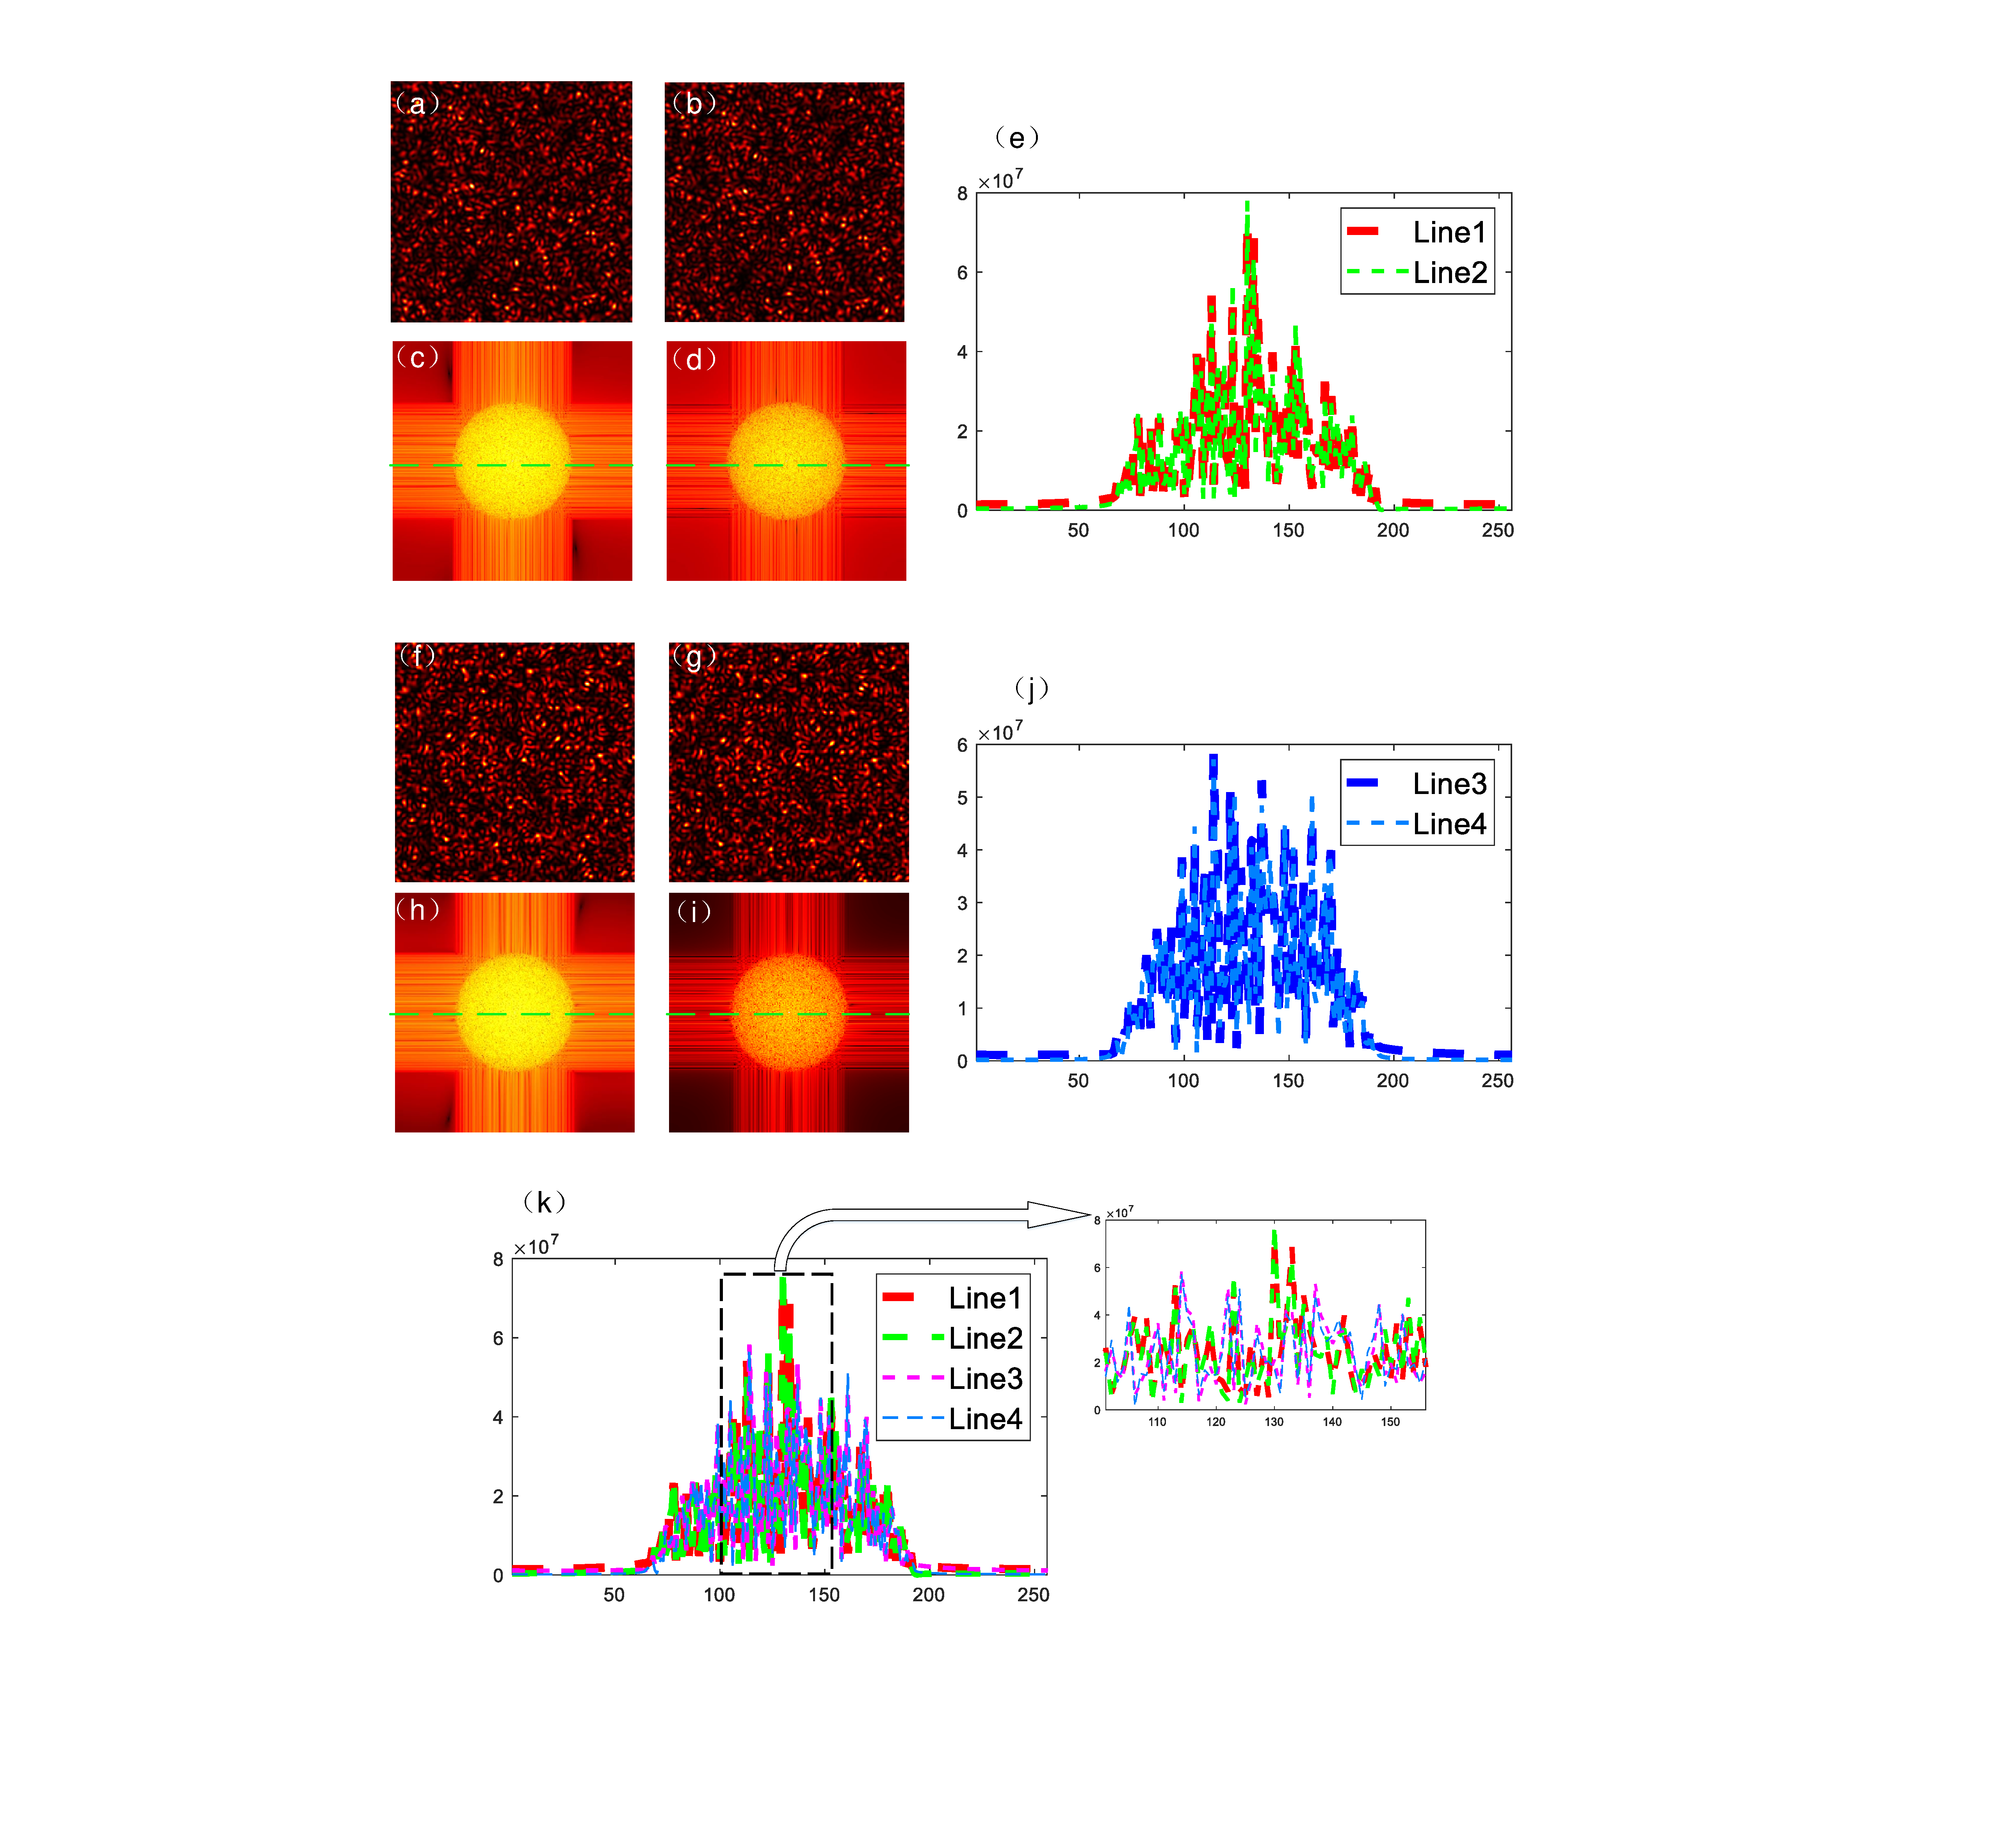
\includegraphics[scale=0.24]{C6.fig2}
	\caption{不同OME范围散斑指纹之间傅里叶振幅信息探索}
	\label{fig:6.2}
\end{figure}
在接下来部分,我们将详细描述散斑分类方法。

\subsection{散斑分类方法I}

\begin{figure}[htp]
	\centering
	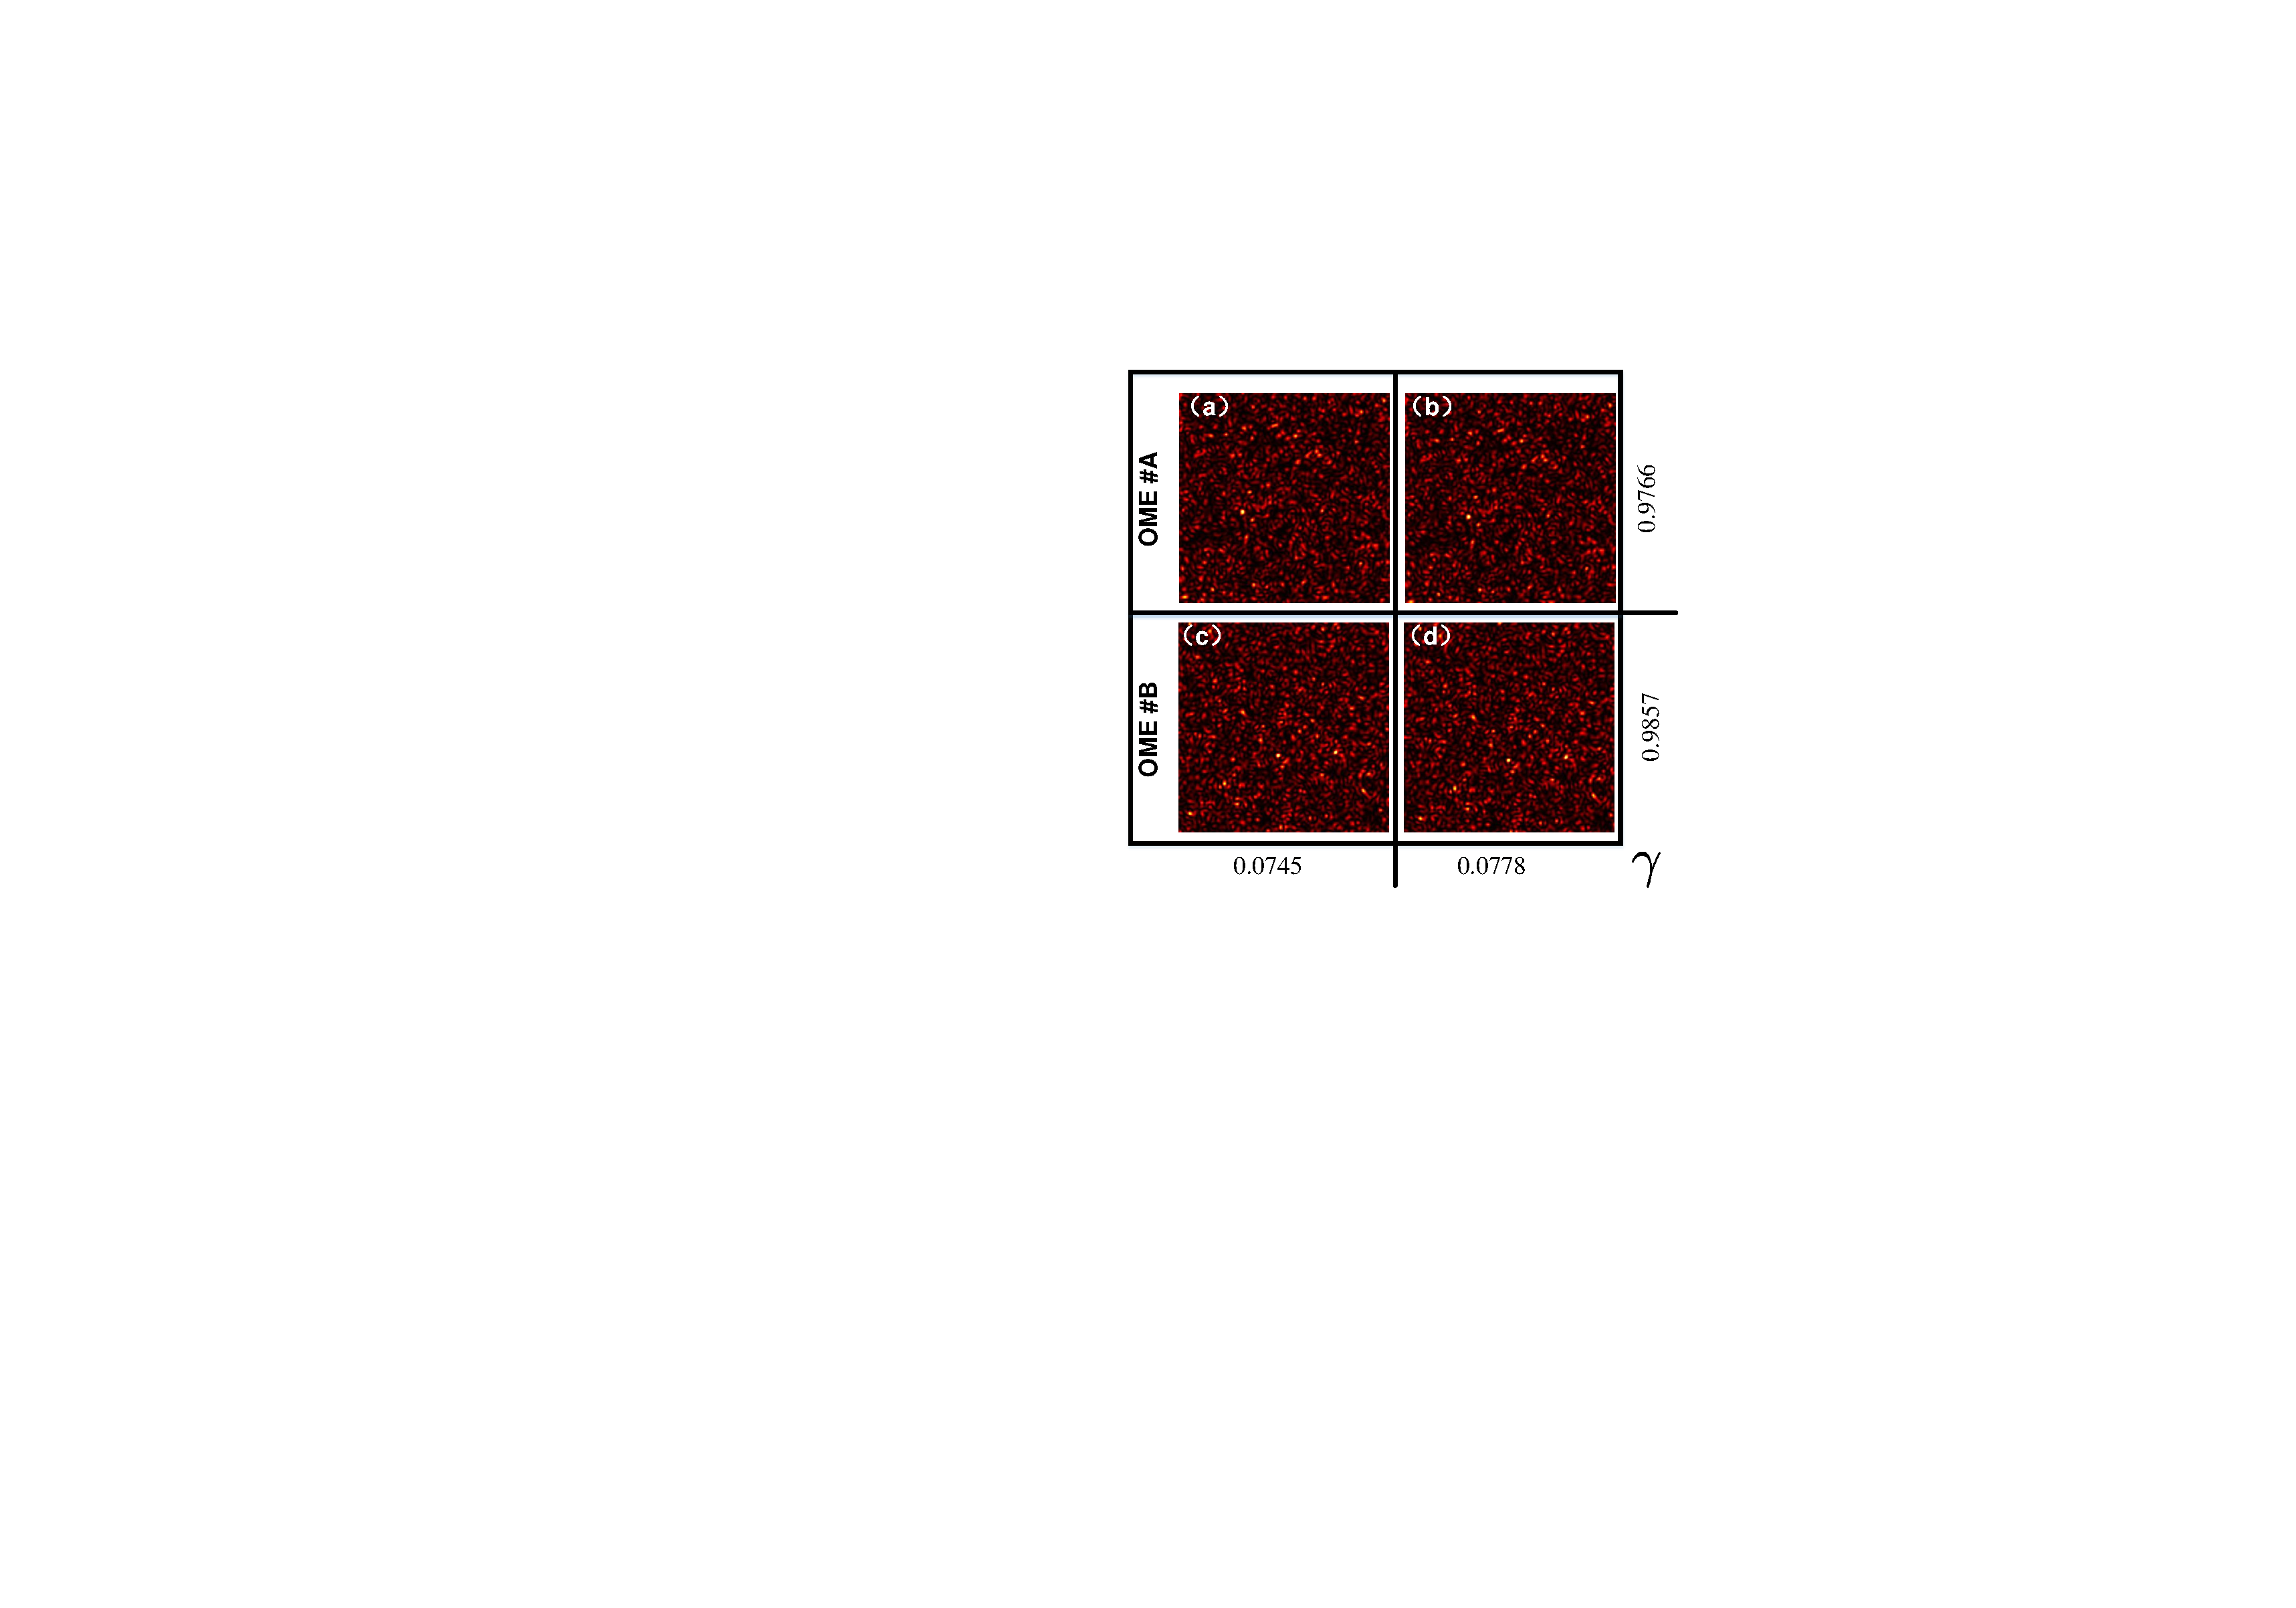
\includegraphics[scale=0.70]{C6.fig5}
	\caption{不同OME范围散斑指纹间相关性探索}
	\label{fig:6.5}
\end{figure}

由于同OME范围内的散斑指纹具有相关性且空间表现为平移,不同OME范围的散斑指纹不相关。受到机器学习图像分类方法的启发,如果我们能获得参考图案作为标准,进行不同散斑的分类,此散斑分类问题将得到有效的解决。由于实际问题中,难以获得散射介质的先验知识或者参考图案,该方法难以实施。但是,当获得散斑指纹后,可以随机的选取$k$个散斑作为参考散斑进行初次分类,然后相应的迭代,进而实现最终的散斑分类。此时设定判定标准,当散斑指纹与参考散斑之间的相关大于阈值且相互之间具有空间平移特点,该散斑指纹与参考散斑属于同一OME范围;当散斑之间的相关稀疏小于阈值或者之间不具空间平移特性时,它们属于不同的光学记忆效应范围。此处,获取散斑指纹与参考散斑之间相关系数的公式为:

\begin{equation}
\begin{aligned}
\gamma (\mu,\nu) = \frac{\sum_{x,y} [w(x,y)- \bar{w}_{\mu,\nu}] [t(x-\mu,y-\nu)- \bar{t}]}{\{ \sum_{x,y} [w(x,y)- \bar{w}(x,y)]^2 \sum_{x,y} [t(x-\mu,y-\nu)- \bar{t}]^2  \}^{0.5}}
\label{eq:6.5}
\end{aligned}
\end{equation}
其中,$w$为散斑指纹,$\bar{t}$为参考图案的平均值,$\bar{w}_{\mu,\nu}$为参考图案区域中$w(x,y)$的平均值。
为了进行探索不OME范围散斑指纹之间相关系数特点,我们进行了相应的仿真,结果如图\ref{fig:6.5}所示。在图\ref{fig:6.5}中,
位于$\mbox{OME} \# \mbox{A}$内散斑(a)和(b)之间的最大相关系数为:$0.9766$;
位于$\mbox{OME} \# \mbox{A}$内散斑(a)和位于$\mbox{OME} \# \mbox{B}$散斑(c)之间的最大相关系数为:$0.0745$;
位于$\mbox{OME} \# \mbox{A}$内散斑(b)和位于$\mbox{OME} \# \mbox{d}$散斑(c)之间的最大相关系数为:$0.0778$;
位于$\mbox{OME} \# \mbox{B}$内散斑(c)和位于$\mbox{OME} \# \mbox{B}$散斑(d)之间的最大相关系数为:$0.9857$。由以上结果可知,位于同一OME范围内的散斑指纹之间的相关系数的最大值往往较高,大于0.1;位于不同OME范围内的散斑之间的相关系数的最大值值较小,通常小于0.1。

于是,在我们所提出的散斑分类方法中将相关系数的最大值作为判据,该阈值为0.1。换而言之,$\gamma (\mu,\nu)$的最大值$\mbox{arg}_{max} \{ \gamma (\mu,\nu) \}$,该值作为判断散斑指纹与参考散斑之间是否属于同一OME范围的标准,即,当$\mbox{arg}_{max} \{ \gamma (\mu,\nu) \} \geq 0.1 $ 时,该散斑指纹与参考散斑属于同一OME范围;当$\mbox{arg}_{max} \{ \gamma (\mu,\nu) \} < 0.1 $ 时,它们属于不同的OME范围。

\subsection{散斑分类方法II}\label{speckle_classify}

受到机器学习和机器视觉相关方法的启发,本小节将会利用多维缩放(Multidimensional scaling,MDS)方法进行散斑分类。MDS是对象集之间距离或差异的直观表示。Warren S. Torgerson首先提出了MDS方法并创造了术语\cite{torgerson_multidimensional_1952}。对象可以是颜色、面孔、地图坐标、政治说服或任何类型的真实或概念体。与不太相似(或距离较长)的对象相比,更相似(或距离更短)的对象在图上更靠近。该图可能由 $p = 1$、$p = 2$或$p = 3$甚至更多维度组成。MDS现在被广泛应用于市场营销、社会学、物理学、政治学和生物学\cite{de_leeuw_modern_2005}。

从技术角度来说,MDS实现散斑图像分类的关键在于如何定量化描述不同散斑之间的相似度,如何将相似度用空间距离的形式进行表示。如上部分所证明,同一OME范围内的散斑在傅里叶域的振幅信息非常接近。当不同的散斑的傅里叶振幅信息相近时,我们定义它们之间的距离越近;当它们的傅里叶振幅信息差异较大时,它们之间的距离信息越远。当获得任何两个散斑指纹之间的空间距离后,该距离信息可以表示为矩阵$D$。

以上所描述的流程可以简化为:\par
1.将$P$个散斑指纹分配给$P$维空间中的任意坐标;\par
2.计算所有点对之间的距离,形成$D$矩阵;\par
3.通过评估应力函数将$\hat{D}$矩阵与输入$D$矩阵进行比较。值越小,两者的对应关系越大;\par
4.调整每个点的坐标到最大应力的最佳方向;\par
5.重复步骤 2 到 4,直到压力不再降低;\par

MDS中的应力函数为:

\begin{equation}
\begin{aligned}
stress_{[u_1,u_2,\ldots, u_r]} =\left( \sum_{\substack{i\neq j = 1,\ldots,r} } (d_{ij}-\Vert u_{i}- u_{j} \Vert ) \right)^{1/2}
\label{eq:6.6}
\end{aligned}
\end{equation}
其中,$d_{ij}$为矩阵$D$中的元素。

为了直观的展示散斑分类方法\Romannum{2};我们进行了相应的仿真,仿真结果如图\ref{fig:6.6}所示。在图\ref{fig:6.6}中,(a)计算不同散斑指纹之间傅里叶域振幅信息的相似程度,并将其转换为矩阵$D$;(b)为将矩阵$D$输入MDS算法,进行优化并且可视化显示空见距离的的结果。由图(a)可以明显看出,此时我们的散斑数据按照不同的OME范围进行排列,然后再实际应用中难以获得此类数据。所获得散斑指纹往往无规律排列,为了验证当我们获得无规律的散斑指纹时,该方法的有效性,我们进行了仿真验证,验证结果如图\ref{fig:6.6}(c)和(d)所示。从图\ref{fig:6.6}(c)可以看出,此时的散斑指纹排列杂乱无序,更符合实际应用情况;从\ref{fig:6.6}(d)可以看出,在此种杂乱无序的散斑指纹序列中,基于MDS散斑分类方法仍然有效。
\begin{figure}[htp]
	\centering
	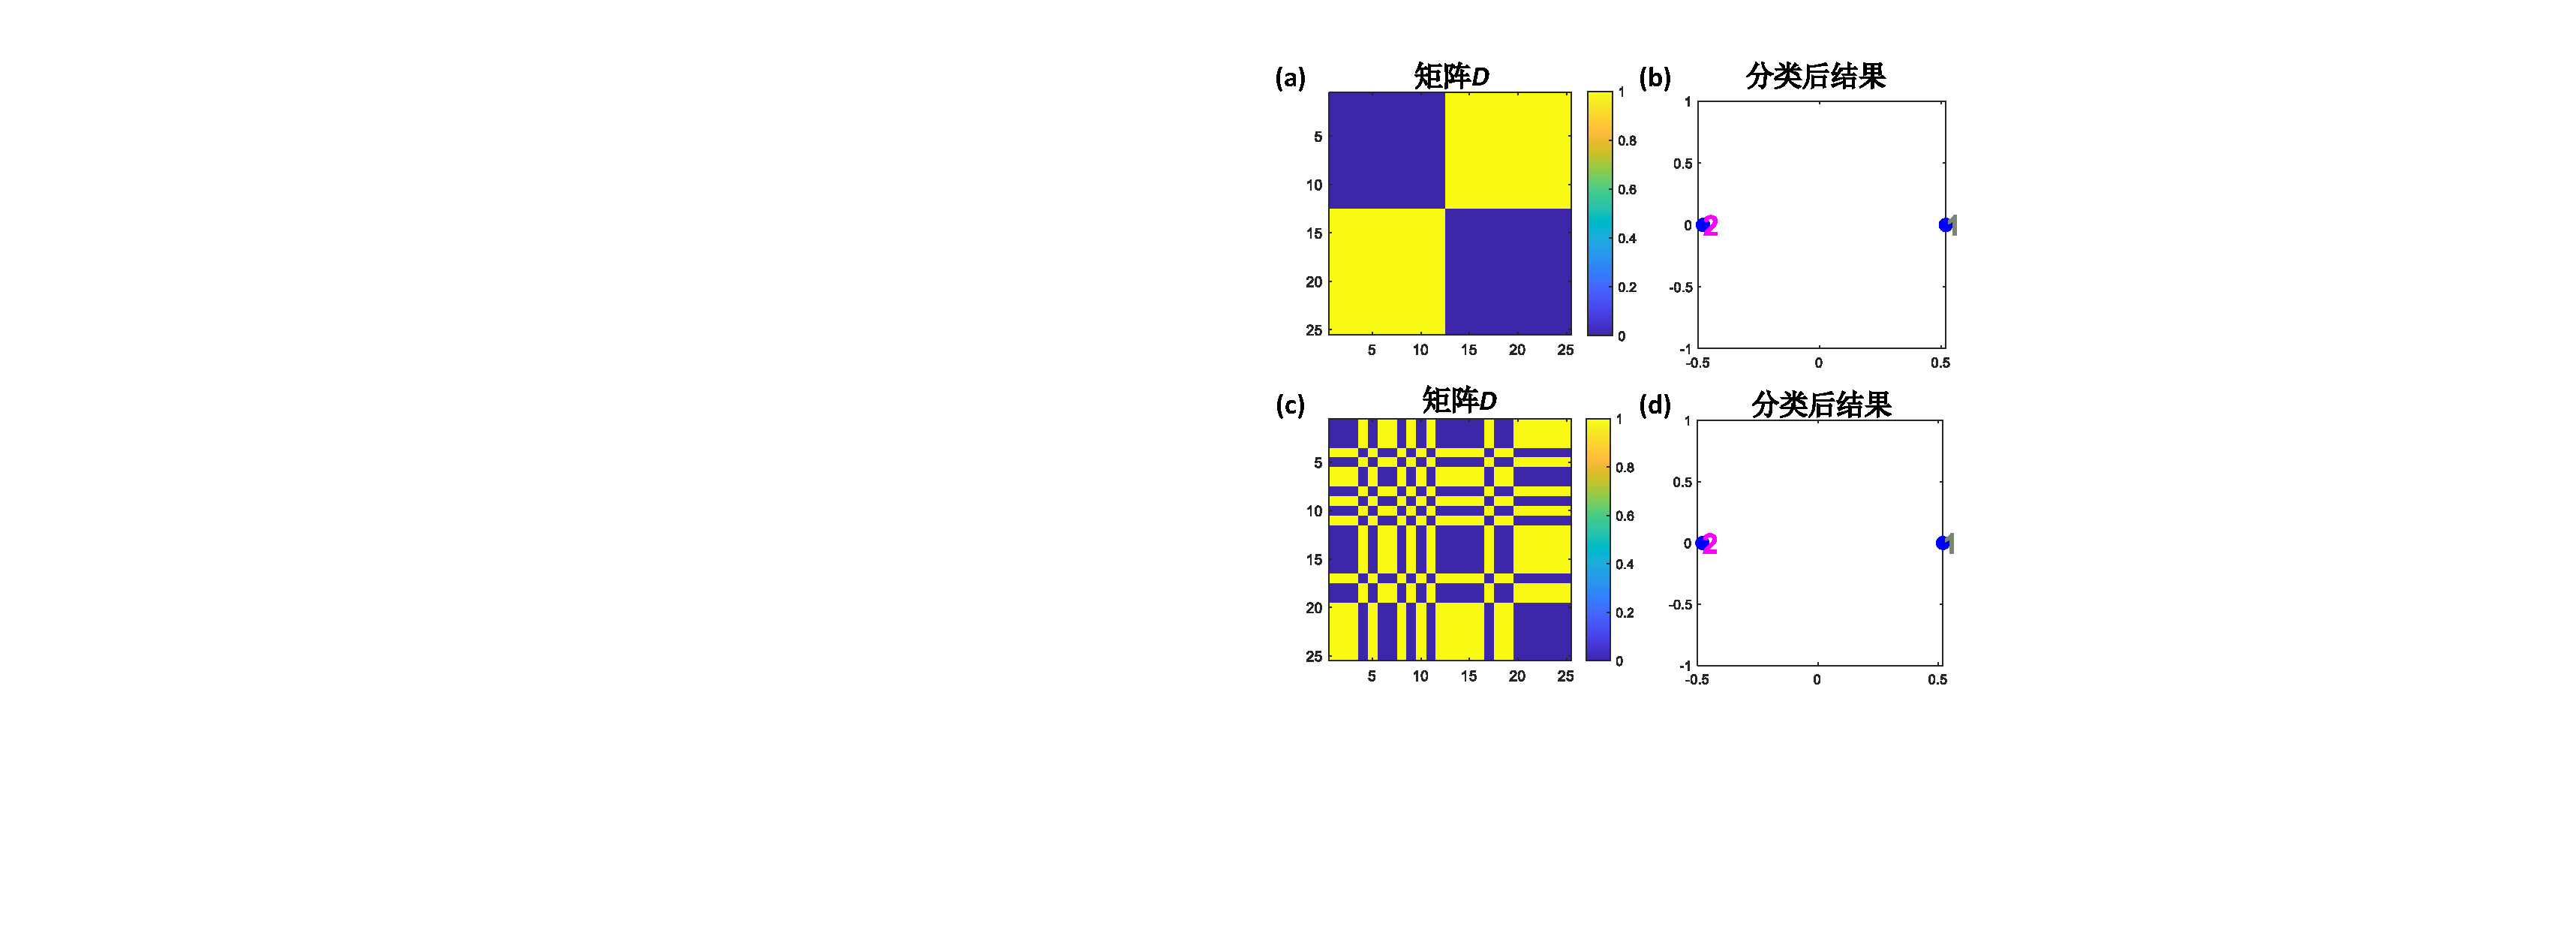
\includegraphics[scale=0.75]{C6.fig6}
	\caption{基于MDS的散斑分类仿真结果}
	\label{fig:6.6}
\end{figure}

在以上两小节中,我们对两种散斑分类方法原理进行阐述,并进行了相关的仿真,验证了它们的有效性。在接下来部分,我们将对成像过程进行相关验证。

\subsection{3D目标成像仿真结果与分析}

上一节我们讨论了两种不同的散斑分类方法,能够有效的散斑指纹进行分类,进而实现不同OME范围目标进行重建。首先,我们对散斑分类方法I进行仿真验证,仿真结果如图\ref{fig:6.3}所示。在图\ref{fig:6.3}中,(a)为进行去混叠后的散斑指纹;(b)为不同OME范围的参考散斑;(c)为进行散斑分类后的两组散斑;(d)为分别不同OME范围图像进行重建;(e)为未执行散斑分类操作所获得的重建结果。对比图\ref{fig:6.3}(d)和(e)结果,可知执行散斑分类后重建图像可以有效的重建目标,未进行散斑分类的重建图案为混叠图案。从图\ref{fig:6.3}所示的结果来看,散斑分类方法能够有效的对图像进行分类,分类后的重建步骤便可以利用第\ref{chap:5}章节中的重建方法。

\begin{figure}[htp]
	\centering
	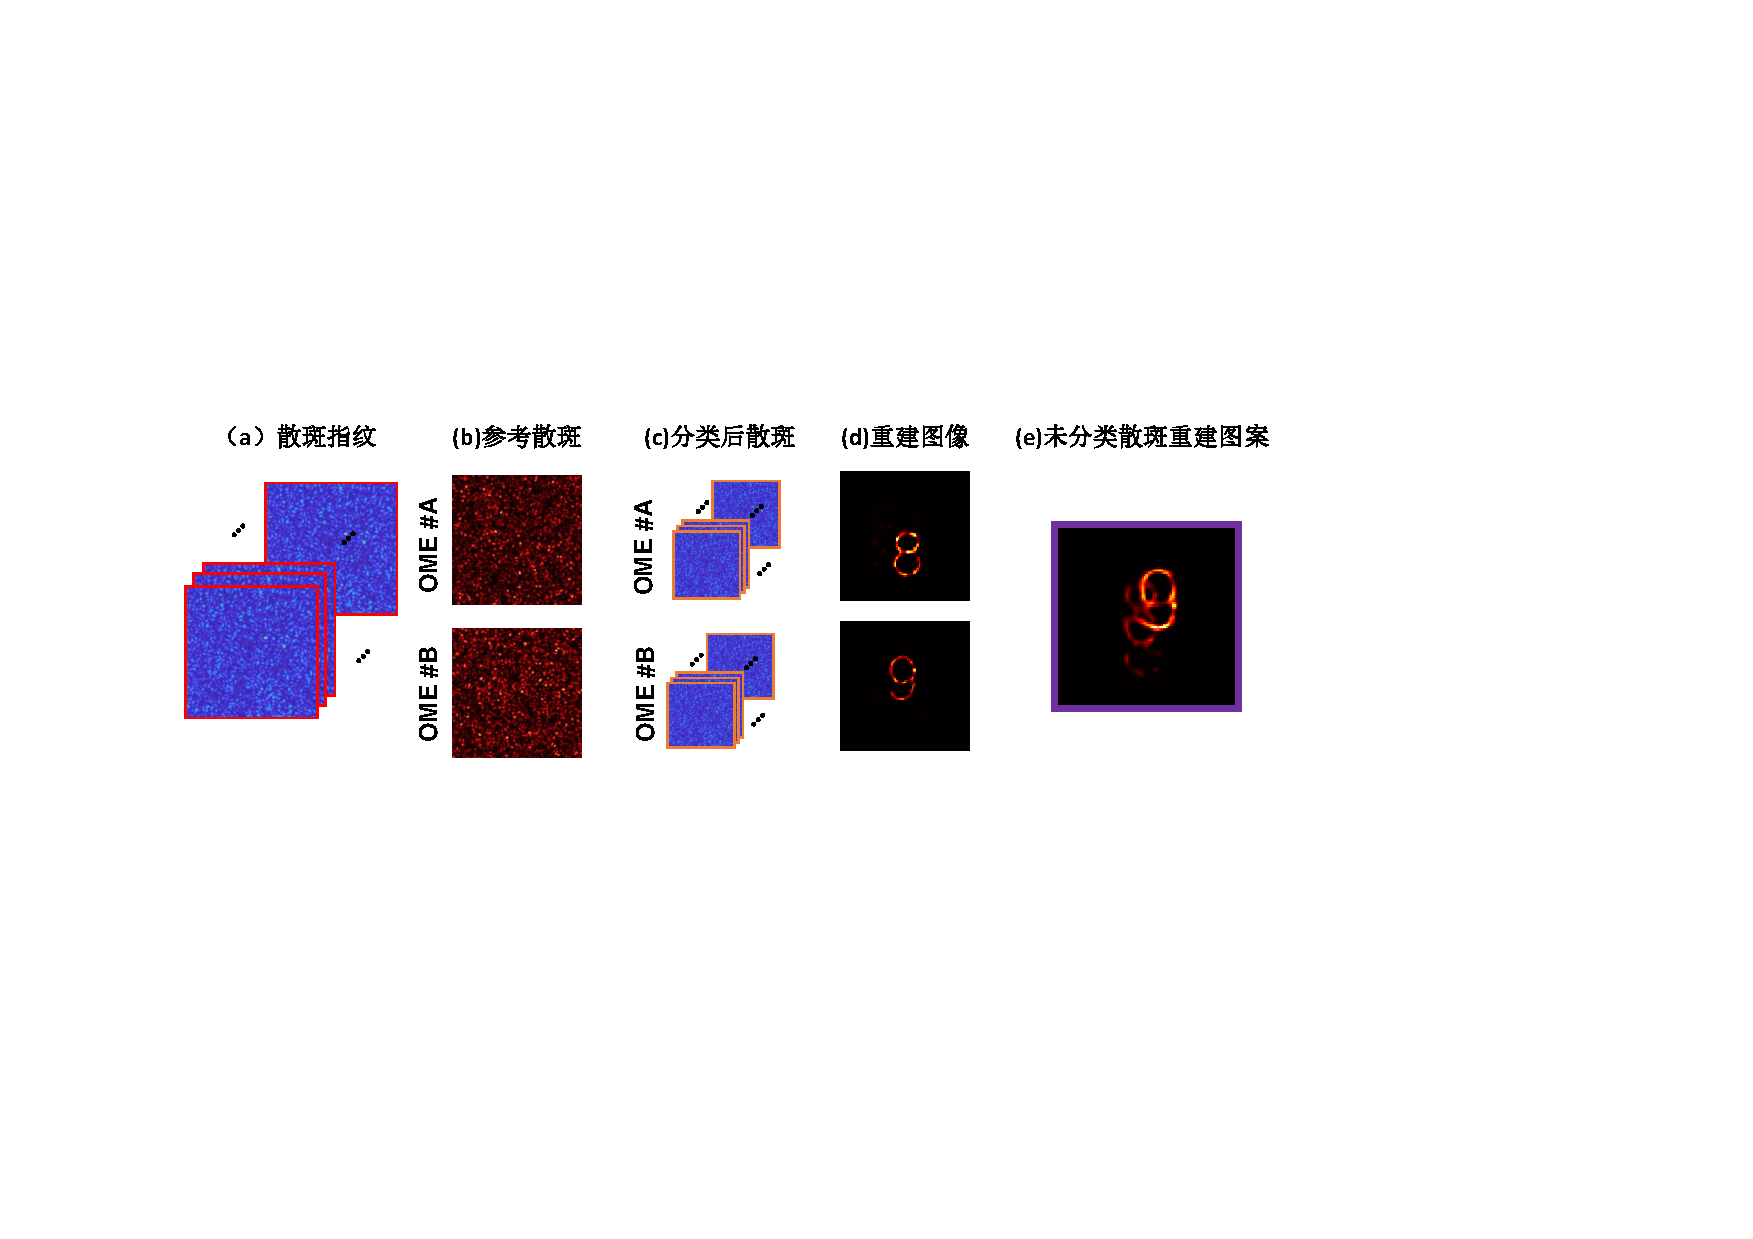
\includegraphics[scale=0.75]{C6.fig3}
	\caption{不同OME范围成像仿真结果}
	\label{fig:6.3}
\end{figure}

\begin{figure}[htp!]
	\centering
	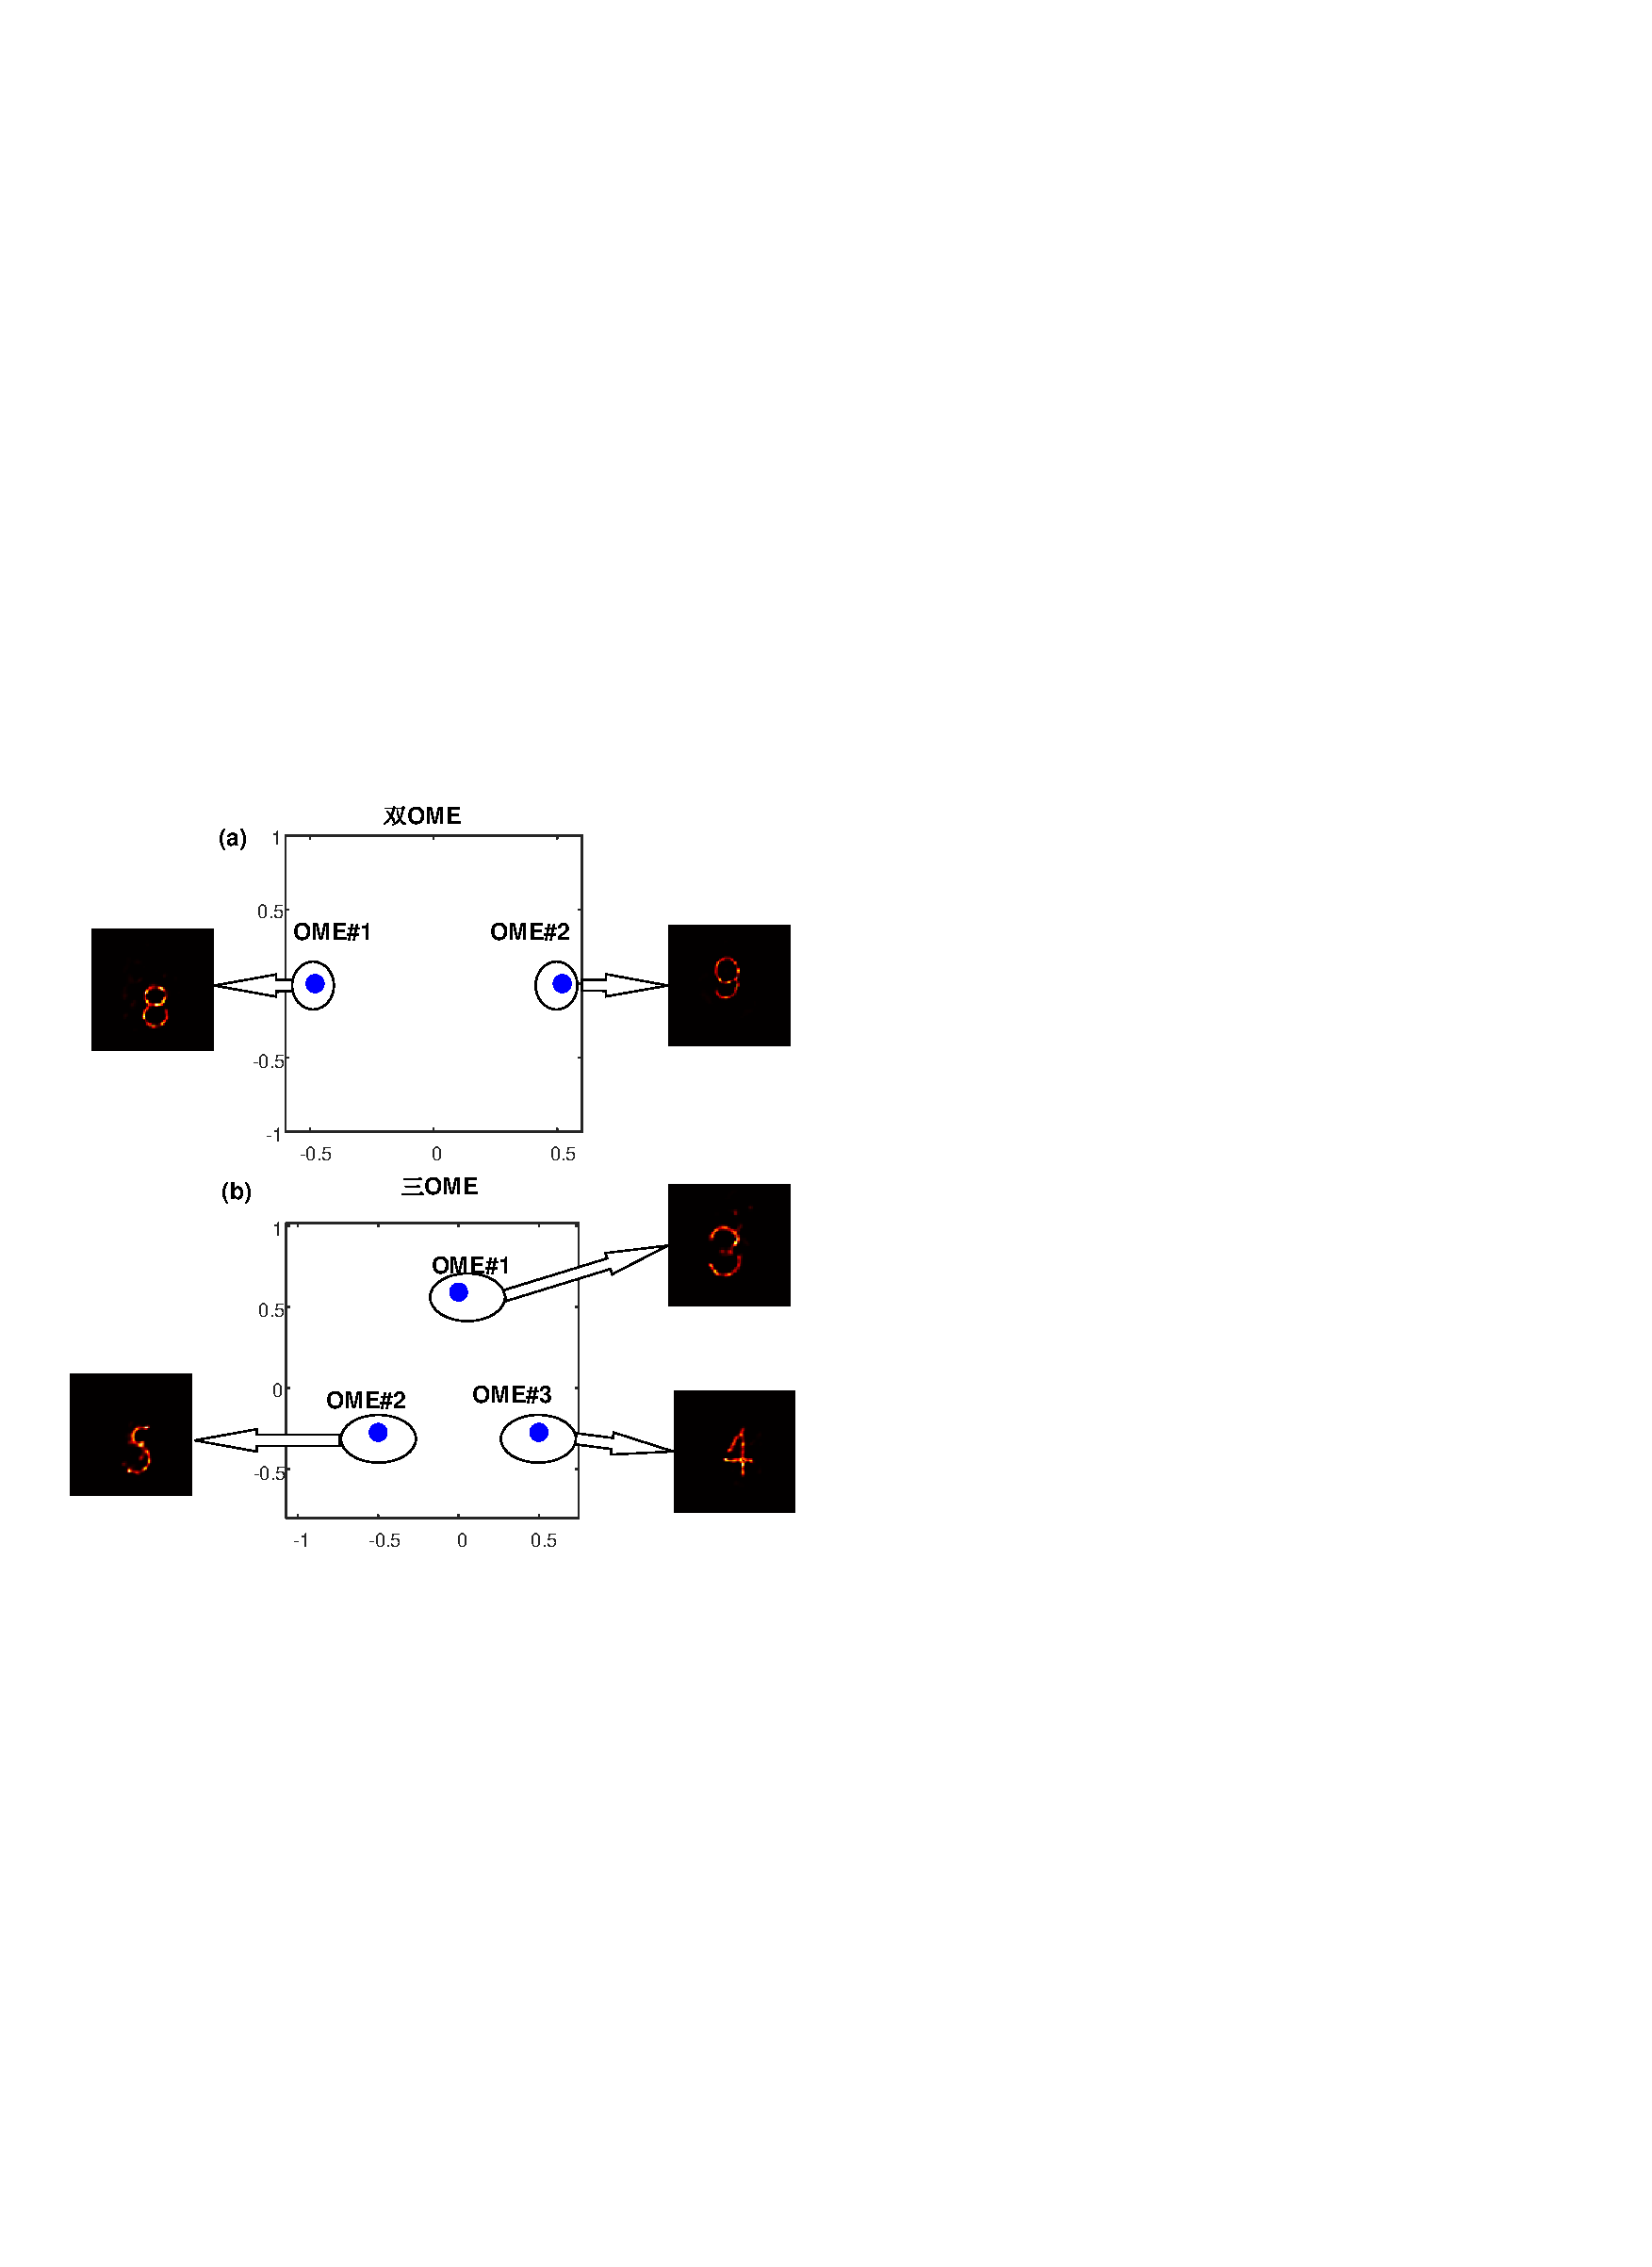
\includegraphics[scale=0.90]{C6.fig4}
	\caption{基于MDS散斑分类散射成像仿真结果}
	\label{fig:6.4}
\end{figure}

如图\ref{fig:6.3}所示结果,当实现散斑分类后,我们便可以有效地重建图像。针对于上部分所描述的散斑分类方法\Romannum{2},将在下部分进行散斑分类的有效性验证。首先,我们仿真生成两个OME范围的不同点光源的散斑指纹,按照上部分所描述的方法,计算不同散斑之间的距离,此距离可以视为散斑的相似程度,获得距离矩阵$D$,将矩阵$D$输入MDS算法,然后获得最终的空间优化结果,双OME范围的基于MDS散斑分类仿真结果如图\ref{fig:6.4}(a)所示。从图\ref{fig:6.4}(a)可以看出,我们所提出的散斑分类方法能够有效地实现散斑图像分类,对分类后的散斑进行图像重建,重建结果也在图中分别进行展示。为了进一步测试对于多OME范围情况下散斑分类的有效性,我们仿真生成三OME的不同点光源的散斑指纹利用MDS算法进行分类,其结果如图\ref{fig:6.4}(b)所示,我们可以看出能够有效的进行散斑分类并进行图像重建。由图\ref{fig:6.4}可知,我们所提出的基于MDS的散斑分类方法能够有效地实现散斑分类。当实现散斑分类后,只需要利用第\ref{chap:5}章节所呈现的FBR算法进行重建图像,其流程类似于图\ref{fig:6.3}所示。为了测试该方法对于复杂目标的重建的有效性,仿真结果如图\ref{fig:6.7}所示。
在图\ref{fig:6.7}所展示的结果中,系统中同时拥有四个目标,且位于不同的OME范围,利用本章所提出的重建算法能够有效地对不同OME范围的目标同时进行重建。从图\ref{fig:6.3}和图\ref{fig:6.7}所示结果,当去混叠后获得不同散斑指纹,如未进行散斑分类步骤,所获得的最终重建结果如图\ref{fig:6.3}(e)所示,不同OME范围的图像重叠,无法成功重建目标。当使用散斑分类方法后,其重建结果如图\ref{fig:6.3}(d)所示,能够分别成功显示不同OME范围的图像。在图\ref{fig:6.7}所示结果中,多OME范围情况下,仍然能够成功同时重建不同OME范围内的图像。

\begin{figure}[htp]
	\centering
	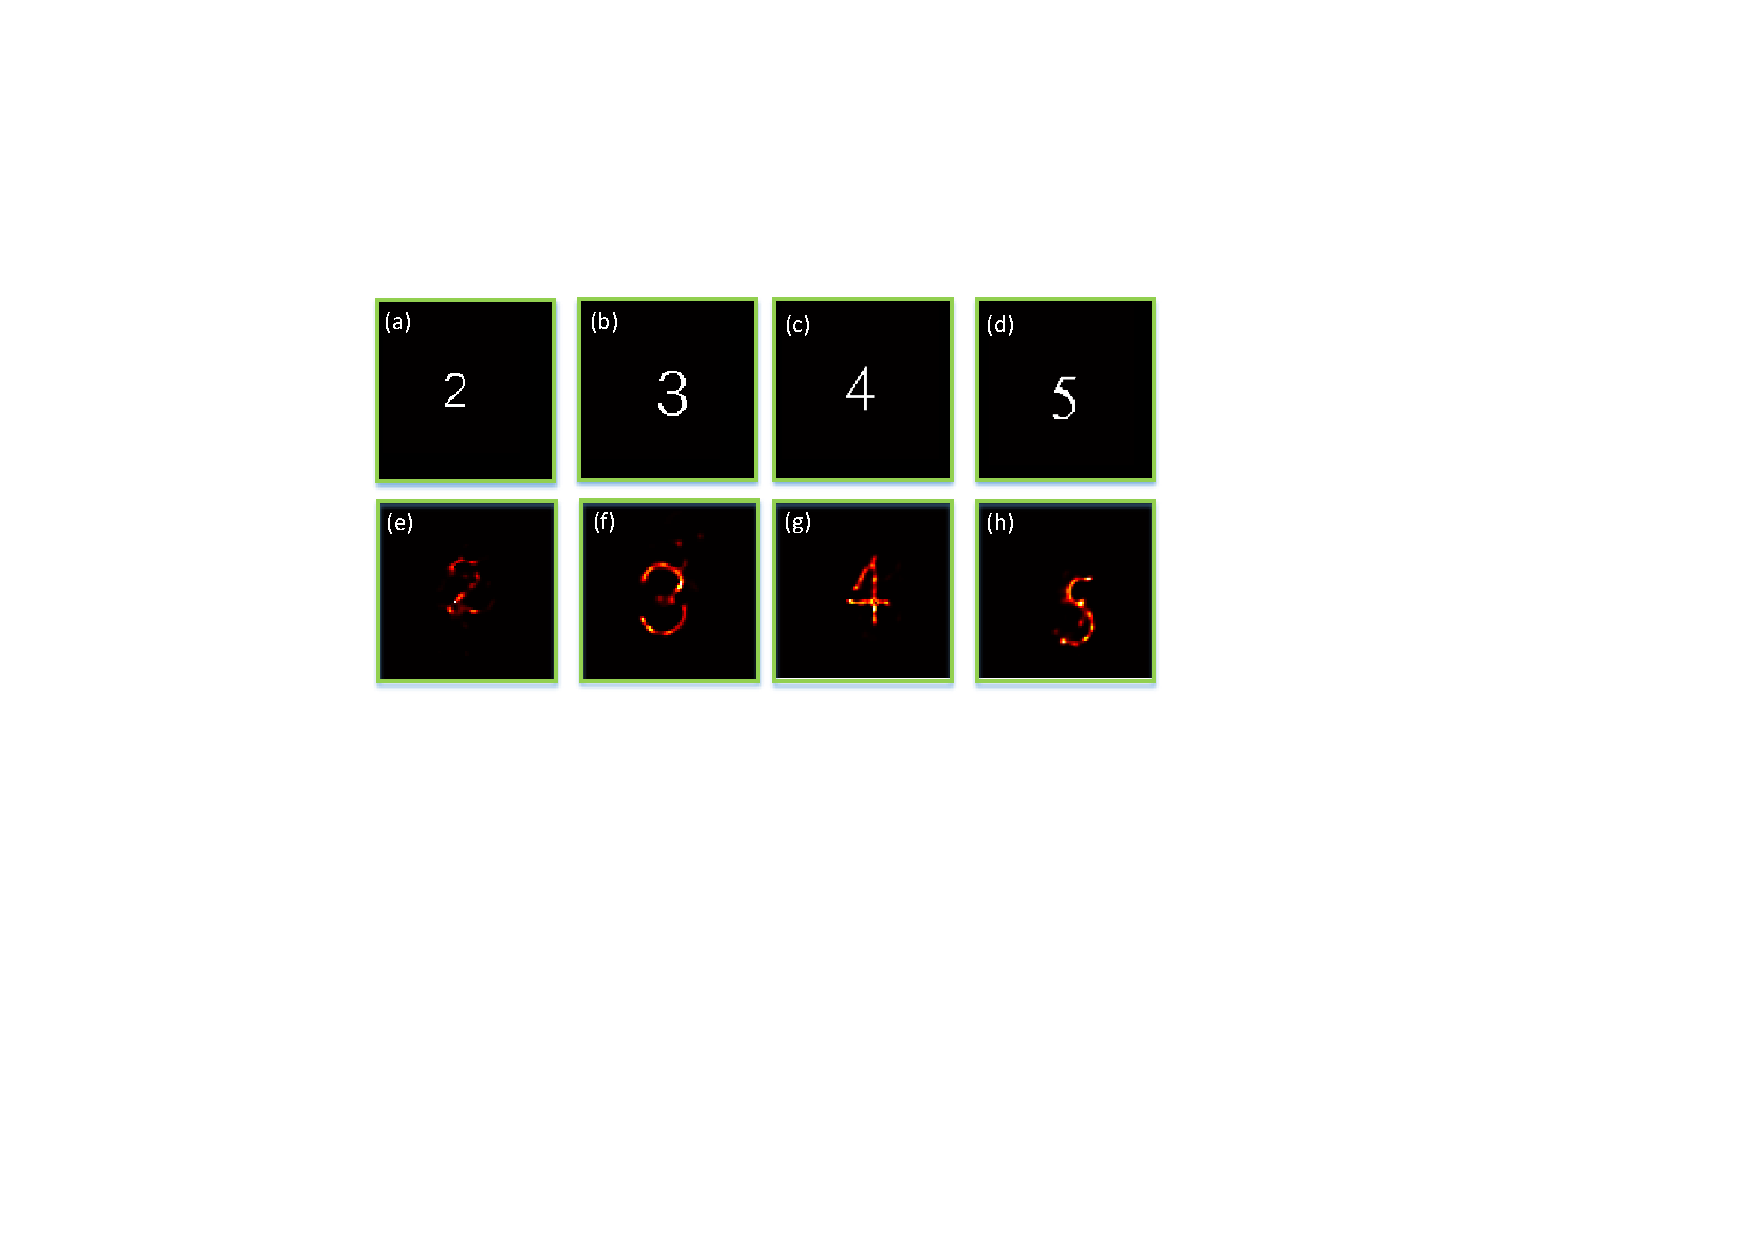
\includegraphics[scale=0.90]{C6.fig7}
	\caption{多OME范围成像仿真结果}
	\label{fig:6.7}
\end{figure}


\section{讨论}

散斑分类方法的核心在于如何将散斑之间的相似性进行量化,量化后如何采用合适算法或者分类框架实现分类,即数据的有效利用。散斑之间的相似信息不仅存在于散斑之间空间相关性、傅里叶域振幅信息的相似性,同时也存在散斑颗粒大小的相似性。当散斑介质一定是,对于特定波长下的散斑照明时,其产生的散斑颗粒大小一定,此类信息也可用于散斑分类。

\section{本章小节}
以上小节我们对透过散射介质3D目标成像方法的立本理论进行了阐述,并进行相应的仿真实验验证,实验结果证明了该方法的有效性。如图\ref{fig:6.3}所示,当未进行散斑分类时所重建的图像未混叠图案,即重建失败。当我们利用散斑分类方法后,能够有效的实现图像重建,有效地分别重建了位于不同OME范围的隐藏目标。

本章所提出的多OME范围散射成像方法,不仅可以实现$XY$平面多OME范围成像,而且可以扩展至$XYZ$三维多OME范围成像。对散斑信息的发掘利用,在不同维度的探索,将更大限度地推动散射成像在众多领域地应用。
